\documentclass[../../main]{subfiles}
\begin{document}
\section{Ros and Simulation}
The Robot Operating System (ROS) is a set of software libraries and tools that help you build robot applications. 
From drivers to state-of-the-art algorithms, and with powerful developer tools, \cite{ros_website}
To effectively approach ROS programming, it's essential to first understand the foundational concepts of ROS and its package management system. 
We will explore key ROS components, including the ROS master, nodes, parameter server, messages, and services. 
Along the way, we will also discuss the necessary steps for installing ROS and initiating work with the ROS master.\\
In the subsequent sections, we will explore the following topics:
\begin{itemize}
\item  Why ROS?
\item  the ROS filesystem level.
\item  ROS computation graph level.
\item  ROS community level.
\end{itemize}
\subsection*{Technical requirements}
To follow this chapter, the only thing you need is a 
standard computer running \href{https://releases.ubuntu.com/20.04/}{Ubuntu 20.04 LTS} or a Debian 10 GNU/Linux 
distribution.
\begin{figure}[h!]
    \centering
    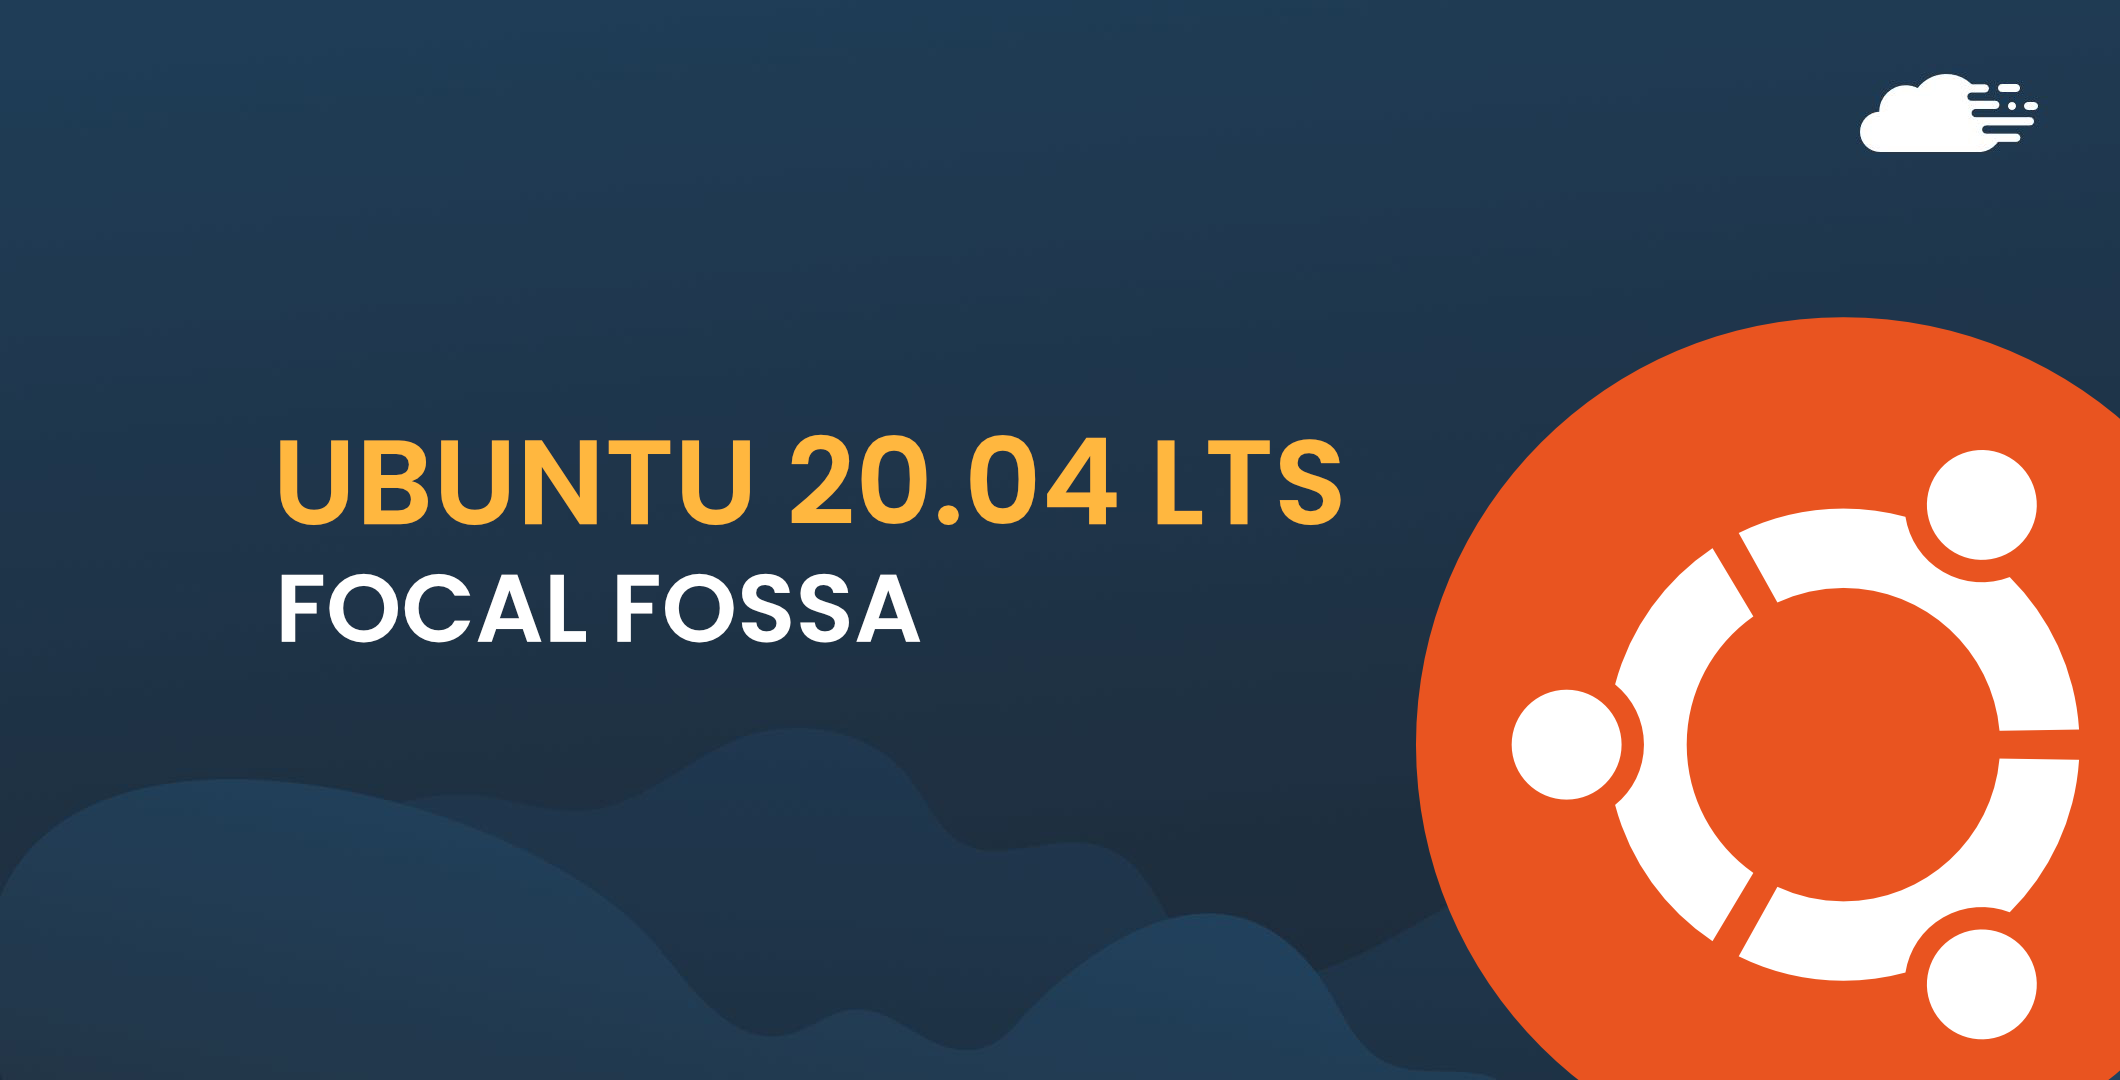
\includegraphics[width=0.7\textwidth]{img/ubuntu.png}
    \caption{Ubuntu 20.04}
\end{figure}
\newpage
\subsection{Why ROS?}\cite{joseph2018mastering}
\emph{Robot Operating System (ROS)} is a flexible framework that provides various tools and
libraries for writing robotic software. It offers several powerful features to help developers
in tasks such as message passing, distributed computing, code reusing, and implementing
state-of-the-art algorithms for robotic applications. The ROS project was started in 2007
by Morgan Quigley and its development continued at Willow Garage, a robotics research
lab for developing hardware and open source software for robots. The goal of ROS was
to establish a standard way to program robots while offering off-the-shelf software
components that can be easily integrated with custom robotic applications. There are
many reasons to choose ROS as a programming framework, and some of them are as
follows:
\subsubsection{High-end capabilities:}ROS comes with ready-to-use functionalities. For example,
    the \\\emph{Simultaneous Localization and Mapping (SLAM)} and \emph{Adaptive Monte
    Carlo Localization (AMCL)} packages in ROS can be used for having autonomous
    navigation in mobile robots, while the \lstinline!MoveIt! package can be used for motion
    planning for robot manipulators. These capabilities can directly be used in our
    robot software without any hassle. In several cases, these packages are enough for
    having core robotics tasks on different platforms. Also, these capabilities are highly
    configurable; we can fine-tune each one using various parameters.
\subsubsection{Tons of tools:} The ROS ecosystem is packed with tons of tools for debugging,
    visualizing, and having a simulation. The tools, such as \emph{rqt\_gui, RViz}, and \emph{Gazebo},
    are some of the strongest open source tools for debugging, visualization, and
    simulation. A software framework that has this many tools is very rare.
\subsubsection{Support for high-end sensors and actuators:} ROS allows us to use different device
    drivers and the interface packages of various sensors and actuators in robotics. Such
    high-end sensors include 3D LIDAR, laser scanners, depth sensors, actuators, and
    more. We can interface these components with ROS without any hassle.
\subsubsection{Inter-platform operability:} The ROS message-passing middleware allows
    communication between different programs. In ROS, this middleware is known
    as nodes. These nodes can be programmed in any language that has ROS client
    libraries. We can write high-haveance nodes in C++ or C and other nodes in Python
    or Java.
\subsubsection{Modularity:}One of the issues that can occur in most standalone robotic
    applications is that if any of the threads of the main code crash, the entire robot
    application can stop. In ROS, the situation is different; we are writing different
    nodes for each process, and if one node crashes, the system can still work.
\subsubsection{Concurrent resource handling:} Handling a hardware resource via more than two
processes is always a headache. Imagine that we want to process an image from a
camera for face detection and motion detection; we can either write the code as a
single entity that can do both, or we can write a single-threaded piece of code for
concurrency. If we want to add more than two features to threads, the application
behavior will become complex and difficult to debug. But in ROS, we can access
devices using ROS topics from the ROS drivers. Any number of ROS nodes can
subscribe to the image message from the ROS camera driver, and each node can
have different functionalities. This can reduce the complexity in computation and
also increase the debugging ability of the entire system.


Most high-end robotics companies are now porting their software to ROS.
This trend is also visible in industrial robotics, in which companies are switching from
proprietary robotic applications to ROS.
Now that we know why it is convenient to study ROS, we can start introducing its core
concepts. There are mainly three levels in ROS: the filesystem level, the computation graph
level, and the community level. We will briefly have a look at each level.
\newpage
\subsection{the ROS filesystem level}
ROS is more than a development framework. We can refer to ROS as a meta-OS, since
it offers not only tools and libraries but even OS-like functions, such as hardware
abstraction, package management, and a developer toolchain. Like a real operating
system, ROS files are organized on the hard disk in a particular manner, as depicted in the
following diagram:
\begin{figure}[ht]
    \centering
    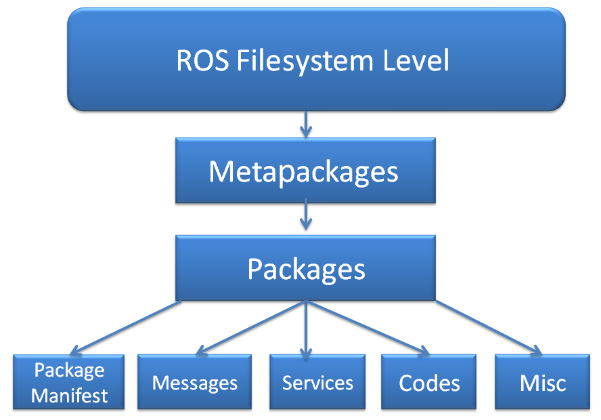
\includegraphics{img/filesystem.jpg}
    \caption{ROS filesystem level}
\end{figure}
Here are the explanations for each block in the filesystem:
\begin{itemize}
\item  \emph{Packages:} The ROS packages are a central element of the ROS software. They
    contain one or more ROS programs (nodes), libraries, configuration files, and so
    on, which are organized together as a single unit. Packages are the atomic build and
    release items in the ROS software.
\item  \emph{Package manifest:} The package manifest file is inside a package and contains
    information about the package, author, license, dependencies, compilation flags,
    and so on. The package.xml file inside the ROS package is the manifest file of
    that package.
\item  \emph{Metapackages:} The term metapackage refers to one or more related packages that
    can be loosely grouped. In principle, metapackages are virtual packages that don't
    contain any source code or typical files usually found in packages.
\item  \emph{Metapackages manifest:} The metapackage manifest is similar to the package
    manifest, with the difference being that it might include packages inside it as
    runtime dependencies and declare an export tag.
\item  \emph{Messages (.msg):} We can define a custom message inside the msg folder inside
    a package (my\_package/msg/MyMessageType.msg). The extension of the
    message file is .msg.
\item  \emph{Services (.srv):} The reply and request data types can be defined inside the srv
    folder inside the package (my\_package/srv/MyServiceType.srv).
\item  \emph{Repositories:} Most of the ROS packages are maintained using a Version Control
    System (VCS) such as Git, Subversion (SVN), or Mercurial (hg). A set of files
    placed on a VCS represents a repository.
\end{itemize}
The following screenshot gives you an idea of the files and folders of a package that we are
going to create in the upcoming sections:
\begin{figure}[ht]
    \centering
    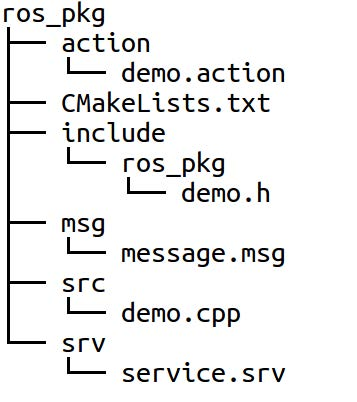
\includegraphics{img/rosfile.jpg}
    \caption{List of files inside the package}
\end{figure}

\subsection{ROS packages}
The typical structure of a ROS package is shown here:
\begin{figure}[ht]
    \centering
    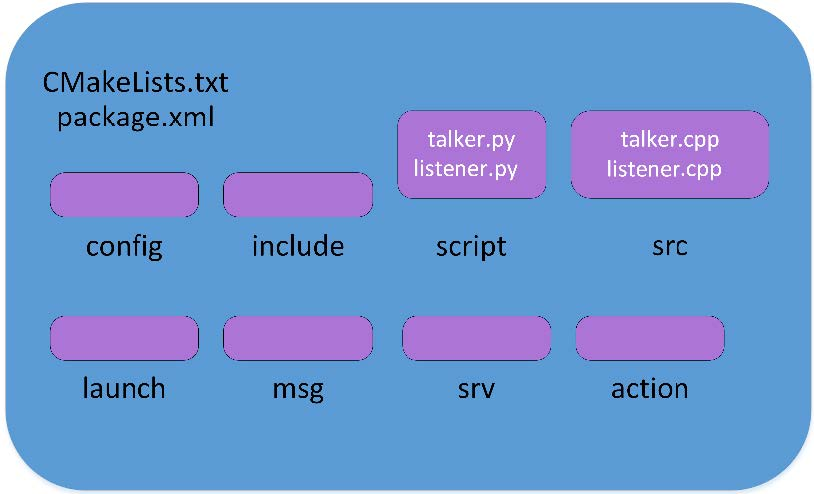
\includegraphics{img/rospkg.jpg}
    \caption{Structure of a typical C++ ROS package}
\end{figure}

\begin{itemize}
    \item \emph{config:} All configuration files that are used in this ROS package are kept in this
    folder. This folder is created by the user and it is a common practice to name the
    folder config as this is where we keep the configuration files.
    \item \emph{include/package\_name:} This folder consists of headers and libraries that we
    need to use inside the package.
    script: This folder contains executable Python scripts. In the block diagram, we
can see two example scripts.
\item \emph{src:} This folder stores the C++ source codes.
\item \emph{launch:} This folder contains the launch files that are used to launch one or more
ROS nodes.
\item \emph{msg:} This folder contains custom message definitions.
\item \emph{srv:} This folder contains the services definitions.
\item \emph{action:} This folder contains the action files.
\item \emph{package.xml:} This is the package manifest file of this package.
\item \emph{CMakeLists.txt:} This file contains the directives to compile the package.
    
\end{itemize}
We need to know some commands for creating, modifying, and working with ROS
packages. Here are some of the commands we can use to work with ROS packages:
\begin{itemize}
\item \emph{catkin\_create\_pkg:} This command is used to create a new package.
\item \emph{rospack:} This command is used to get information about the package in the
filesystem.
\item \emph{catkin\_make:} This command is used to build the packages in the workspace.
\item \emph{rosdep:} This command will install the system dependencies required for this
package.
\end{itemize}
To work with packages, ROS provides a bash-like command called rosbash \\
(http://wiki.ros.org/rosbash), which can be used to navigate and manipulate the
ROS\\
package. Here are some of the rosbash commands:

\begin{itemize}
    \item
    \emph{roscd:} This command is used to change the current directory using a
      package name, stack name, or a special location. If we give the
      argument a package name, it will switch to that package folder.
    \item
    \emph{roscp:} This command is used to copy a file from a package.
    \item
    \emph{rosed:} This command is used to edit a file using the vim editor.
    \item
    \emph{rosrun:} This command is used to run an executable inside a package.
    \end{itemize}
    The definition of package.xml in a typical package is shown in the following
    code:
        \begin{codebox}[]{ Typical ROS Package.xml}    
            \begin{minted}{xml}
            <?xml version="1.0"?>
            <package>
            <name>hello world</name>
            <vrsion>0.0.1</version>
            <description>The hello world package</description>
            <maintainer email="example@gmail.com">example</maintainer>
            <buildtool_depend>catkin</buildtool_depend>
            <buildtool_depend>roscpp</build_depend>
            <build_depend>rospy</build_depend>
            <build_depend>std_msgs</build_depend>
            <run_depend>roscpp</run_depend>
            <run_depend>rospy</run_depend>
            <run_depend>std_msgs</run_depend>
            <export>
            </export> </package>
        \end{minted}
    \end{codebox}

        The package.xml file also contains information about the compilation.\\ The \texttt{<build\_
        depend></build\_depend>} tag includes the packages that are necessary for building
        the source code of the package. The packages inside the \texttt{<run\_depend></run\_
        depend>} tags are necessary for running the package node at runtime.
\subsection{ROS metapackages}
Metapackages are specialized packages that require only one file; that is, a package.xml
file.
Metapackages simply group a set of multiple packages as a single logical package. In the
package.xml file, the metapackage contains an export tag, as shown here:
\begin{codebox}[]{Defining a ROS Metapackage with the package.xml File}
    \begin{minted}{xml}
    <export>
    <metapackage/>
    </export>
\end{minted}
    \end{codebox}
Also, in metapackages, there are no \texttt{<buildtool\_depend>} dependencies for catkin;
there are only \texttt{<run\_depend>} dependencies, which are the packages that are grouped
inside the metapackage.\\
\\
The ROS navigation stack is a good example of somewhere that contains metapackages. If
ROS and its navigation package are installed, we can try using the following command by
switching to the navigation metapackage folder:
\begin{codebox}[]{Navigating to the ROS Navigation Metapackage with roscd}
    \begin{minted}{bash}
        roscd navigation
    \end{minted}
    \end{codebox}
    Open package.xml using your text editor (gedit, in the following case):

    \begin{codebox}[]{Opening the package.xml File Using a Text Editor }
        \begin{minted}{xml}
    gedit package.xml
        \end{minted}
        \end{codebox}

        This is a lengthy file; here is a stripped-down version of it:
\begin{codebox}[]{Structure of the package.xml metapackage}
        \begin{minted}{xml}
            <?xml version="1.0"?>
            <package>
            <name>navigation</name>
            <version>l. 14. O</version>
            <description>
            A 2D navigation stack that takes in information from odometry, sensor
            streams, and a goal pose and outputs safe velocity commands that are sent
            to a mobile base.
            </description>
            <url>http : //wiki.ros.org/navigation</url>
            <buildtool_depend>catkin</buildtool_depend>
            <run_depend>amcl</run_depend>
            ...
            <export>
            <metapackage/>
            </export>
            </package>
        \end{minted}
        % \caption{Structure of the package.xml metapackage}
    \end{codebox}

    This file contains several pieces of information about the package, such as a brief
description, its dependencies, and the package version.

\subsection{ROS messages}
ROS nodes can write or read data of various types. These different types of data are
described using a simplified message description language, also called ROS messages.
These data type descriptions can be used to generate source code for the appropriate
message type in different target languages.
Even though the ROS framework provides a large set of robotic-specific messages that
have already been implemented, developers can define their own message type inside their
nodes.
The message definition can consist of two types: \texttt{fields} and \texttt{constants}. The field is
split into field types and field names. The field type is the data type of the transmitting
message, while the field name is the name of it.

Here is an example of message definitions:
\begin{codebox}[]{Example of ROS Message Definitions: Fields and Data Types}
    \begin{minted}{bash}
        int32 number
    \end{minted}
    \begin{minted}{bash}
        string name
    \end{minted}
    \begin{minted}{bash}
        float32 speed
    \end{minted}
    \end{codebox}
Here, the first part is the field type and the second is the field name. The field type is
the data type, and the field name can be used to access the value from the message. For
example, we can use msg.number to access the value of the number from the message.
\newpage
Here is a table showing some of the built-in field types that we can use in our message:

\begin{table}[ht]
    \centering
\begin{tcolorbox}[
    colback=red!5!white,colframe=red!75!black,
    title={\textbf{Built-in Field Types for Message Definition}},
    fonttitle=\bfseries, coltitle=white, width=\linewidth
]
    \begin{tabular}{|c|c|c|c|}
    \hline
    \textbf{Primitive type} & \textbf{Serialization} & \textbf{C++} & \textbf{Python} \\ \hline
    bool (1) & Unsigned 8-bit int & uint8\_t (2) & bool \\ \hline
    int8 & Signed 8-bit int & int8\_t & int \\ \hline
    uint8 & Unsigned 8-bit int & uint8\_t & int (3) \\ \hline
    int16 & Signed 16-bit int & int16\_t & int \\ \hline
    uint16 & Unsigned 16-bit int & uint16\_t & int \\ \hline
    int32 & Signed 32-bit int & int32\_t & int \\ \hline
    uint32 & Unsigned 32-bit int & uint32\_t & int \\ \hline
    int64 & Signed 64-bit int & int64\_t & long \\ \hline
    uint64 & Unsigned 64-bit int & uint64\_t & long \\ \hline
    float32 & 32-bit IEEE float & float & float \\ \hline
    float64 & 64-bit IEEE float & double & float \\ \hline
    string & ascii string (4) & std::string & string \\ \hline
    time & secs/nsecs unsigned 32-bit ints & ros::Time & rospy.Time \\ \hline
    duration & secs/nsecs signed 32-bit ints & ros::Duration & rospy.Duration \\ \hline
    \end{tabular}
    \caption{Primitive types and their serialization in C++ and Python.}
    \label{tab:my_label}
\end{tcolorbox}
\end{table}

ROS provides a set of complex and more structured message files that are designed to cover a specific application's necessity, such as exchanging common geometrical (geometry\_msgs) or sensor (sensor\_msgs) information. These messages are composed of different primitive types. A special type of ROS message is called a message header. This header can carry information, such as time, frame of reference or frame\_id, and sequence number. Using the header, we will get numbered messages and more clarity about which component is sending the current message. The header information is mainly used to send data such as robot joint transforms. Here is the definition of the header:
\begin{codebox}[]{ROS Message Header: Sequence, Timestamp, and Frame ID}
\begin{minted}{bash}
    uint32 seq
\end{minted}
\begin{minted}{bash}
    time stamp
\end{minted}
\begin{minted}{bash}
    string frame_id
\end{minted}
\end{codebox}

The rosmsg command tool can be used to inspect the message header and the field types.
The following command helps view the message header of a particular message:
\begin{minted}{bash}
    rosmsg show std_msgs/Header
\end{minted}
This will give you an output like the preceding example's message header. We will look
at the \texttt{rosmsg} command and how to work with custom message definitions later in this
chapter(\cref{message}).

\subsection{The ROS services}
ROS services are a type of request/response communication between ROS nodes. One node will send a request and wait until it gets a response from the other. Similar to the message definitions when using the .msg file, we must define the service definition in another file called .\texttt{srv}, which must be kept inside the \texttt{srv} subdirectory of the package.

An example service description format is as follows:

\begin{codebox}[]{ROS Services: Request and Response}
    
    \begin{minted}[style=default]{bash}
        #Request message type
        string req
        ---
        #Response message type
        string res
    \end{minted}
    \end{codebox}
The first section is the message type of the request, which is separated by ---, while the
next section contains the message type of the response. In these examples, both Request
and Response are strings.
\subsection{the ROS computation graph level}
Computation in ROS is done using a network of ROS nodes. This computation network is called the computation graph. The main concepts in the computation graph are ROS \textbf{nodes}, \textbf{master}, \textbf{parameter server}, \textbf{messages}, \textbf{topics}, \textbf{services}, and \textbf{bags}. Each concept in the graph is contributed to this graph in different ways.

The ROS communication-related packages, including core client libraries, such as roscpp and rospython, and the implementation of concepts, such as topics, nodes, parameters, and services, are included in a stack called ros\_comm (http://wiki.ros.org/ros\_comm).
\\
This stack also consists of tools such as rostopic, rosparam, rosservice, and rosnode to introspect the preceding concepts.
\\
The ros\_comm stack contains the ROS communication middleware packages, and these packages are collectively called the \textbf{ROS graph layer}.
\begin{figure}[ht]
    \centering
    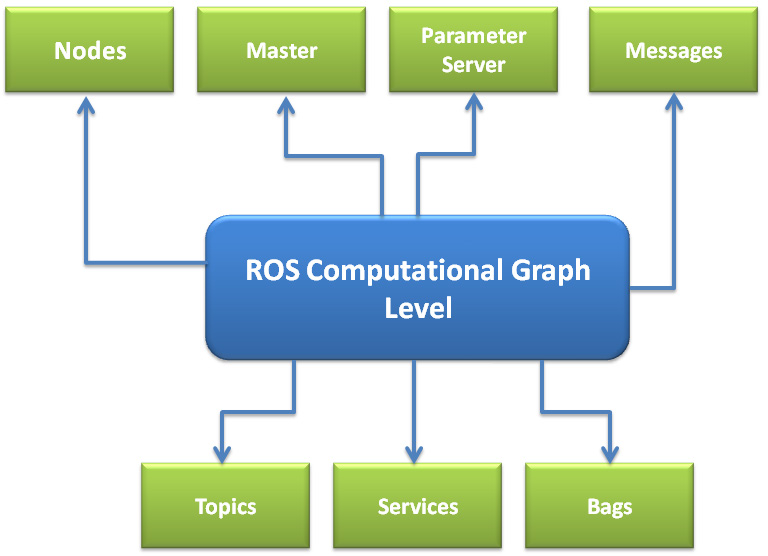
\includegraphics{img/rosgraph.jpg}
    \caption{Structure of the ROS graph layer}
\end{figure}
\newpage
\subsubsection{Nodes}
Nodes are the processes that have computation. Each ROS node is written
using ROS client libraries. Using client library APIs, we can implement different
ROS functionalities, such as the communication methods between nodes, which
is particularly useful when the different nodes of our robot must exchange
information between them. One of the aims of ROS nodes is to build simple
processes rather than a large process with all the desired functionalities. Being
simple structures, ROS nodes are easy to debug.
\subsubsection{Master}
The ROS master provides the name registration and lookup processes for
the rest of the nodes. Nodes will not be able to find each other, exchange messages,
or invoke services without a ROS master. In a distributed system, we should run
the master on one computer; then, the other remote nodes can find each other by
communicating with this master.
\subsubsection{Parameter server}
The parameter server allows you to store data in a central
location. All the nodes can access and modify these values. The parameter server is
part of the ROS master.
\subsubsection{Topics}
Each message in ROS is transported using named buses called topics. When
a node sends a message through a topic, then we can say the node is publishing a
topic. When a node receives a message through a topic, then we can say that the
node is subscribing to a topic. The publishing node and subscribing node are not
aware of each other's existence. We can even subscribe to a topic that might not
have any publisher. In short, the production of information and its consumption are
decoupled. Each topic has a unique name, and any node can access this topic and
send data through it so long as they have the right message type.
\subsubsection{Logging}
ROS provides a logging system for storing data, such as sensor data,
which can be difficult to collect but is necessary for developing and testing robot
algorithms. These are known as bagfiles. Bagfiles are very useful features when we're
working with complex robot mechanisms.

The following graph shows how the nodes communicate with each other using topics:

\begin{figure}[ht]
    \centering
    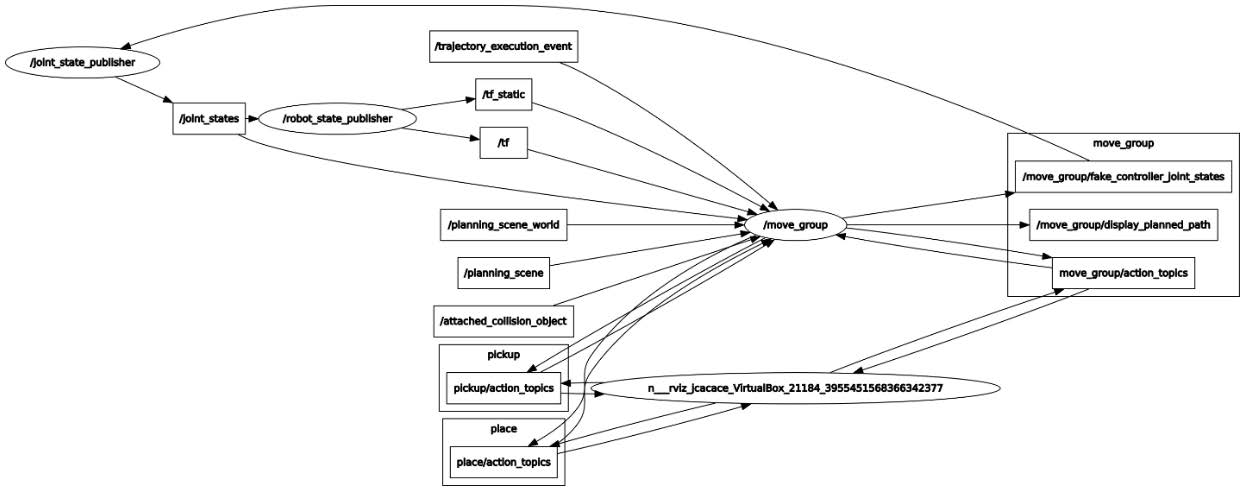
\includegraphics{img/rqt_graph.jpg}
    \caption{Graph of communication between nodes using topics}
\end{figure}
The topics are represented by rectangles, while the nodes are represented by ellipses. The messages and parameters are not included in this graph. These kinds of graphs can be generated using a tool called \textbf{rqt\_graph} (http://wiki.ros.org/rqt\_graph).
\subsection{ROS nodes}
ROS nodes have computations using ROS client libraries such as \texttt{roscpp} and \texttt{rospy}. A robot might contain many nodes; for example, one node processes camera images, one node handles serial data from the robot, one node can be used to compute odometry, and so on.

Using nodes can make the system fault-tolerant. Even if a node crashes, an entire robot system can still work. Nodes also reduce complexity and increase debug-ability compared to monolithic code because each node is handling only a single function.

All running nodes should have a name assigned to help us identify them. For example, /camera\_node could be the name of a node that is broadcasting camera images.

There is a rosbash tool for introspecting ROS nodes. The \texttt{rosnode} command can be used to gather information about an ROS node. Here are the usages of \textbf{rosnode}:

\begin{itemize}
    \item \texttt{rosnode info [node\_name]}: This will print out information about the node.
    \item \texttt{rosnode kill [node\_name]}: This will kill a running node.
    \item \texttt{rosnode list}: This will list the running nodes.
    \item  \texttt{rosnode machine [machine\_name]:} This will list the nodes that are running
    on a particular machine or a list of machines.
    \item  \texttt{rosnode ping:} This will check the connectivity of a node.
    \item  \texttt{rosnode cleanup:} This will purge the registration of unreachable nodes.
\end{itemize}
some example nodes that use the roscpp client and discuss how
ROS nodes that use functionalities such ROS topics, service, messages, and actionlib
work.
\subsection{ROS messages}\label{message}
messages are simple data structures that contain field types. ROS messages support standard primitive data types and arrays of primitive types.

We can access a message definition using the following method. For example, to access std\_msgs/msg/String.msg when we are using the roscpp client, we must include std\_msgs/String.h for the string message definition.

In addition to the message data type, ROS uses an MD5 checksum comparison to confirm whether the publisher and subscriber exchange the same message data types.

ROS has a built-in tool called \texttt{rosmmsg} for gathering information about ROS messages. Here are some parameters that are used along with \texttt{rosmmsg}:
\begin{itemize}
    \item \texttt{rosmmsg show [message\_type]}: This shows the message's description.
    \item \texttt{rosmmsg list}: This lists all messages.
    \item \texttt{rosmmsg md5 [message\_type]}: This displays md5sum of a message.
    \item \texttt{rosmmsg package [package\_name]}: This lists messages in a package.
    \item \texttt{rosmmsg packages [package\_1] [package\_2]}: This lists all packages that contain messages.
\end{itemize}
\newpage
\subsection{ROS topics}
Using topics, the ROS communication is unidirectional. Differently, if we want a direct
request/response communication, we need to implement ROS services.
The ROS nodes communicate with topics using a TCP/IP-based transport known as \textbf{TCPROS}. This method is the default transport method used in ROS. Another type of communication is \textbf{UDPROS}, which has low latency and loose transport and is only suited for teleoperations.
The ROS topic tool can be used to gather information about ROS topics. Here is the syntax of this command:
\begin{itemize}
    \item \textbf{rostopic bw /topic}: This command will display the bandwidth being used by the given topic.
    \item \textbf{rostopic echo /topic}: This command will print the content of the given topic in a human-readable format. Users can use the -p option to print data in CSV format.
    \item \textbf{rostopic find /message\_type}: This command will find topics using the given message type.
    \item \textbf{rostopic hz /topic}: This command will display the publishing rate of the given topic.
    \item \textbf{rostopic info /topic}: This command will print information about an active topic.
    \item \textbf{rostopic list}: This command will list all the active topics in the ROS system.
    \item \textbf{rostopic pub /topic message\_type args}: This command can be used to publish a value to a topic with a message type.
    \item \textbf{rostopic type /topic}: This will display the message type of the given topic.
\end{itemize}

\subsection{ROS services}
In ROS services, one node acts as a ROS server in which the service client can request the service from the server. If the server completes the service routine, it will send the results to the service client. For example, consider a node that can provide the sum of two numbers that has been received as input while implementing this functionality through an ROS service. The other nodes of our system might request the sum of two numbers via this service. In this situation, topics are used to stream continuous data flows.

The ROS service definition can be accessed by the following method. For example, \texttt{my\_package/srv/Image.srv} can be accessed by \texttt{my\_package/Image}.

In ROS services, there is an MD5 checksum that checks in the nodes. If the sum is equal, then only the server responds to the client.

There are two ROS tools for gathering information about the ROS service. The first tool is \textbf{rossrv}, which is similar to \textbf{rosmmsg}, and is used to get information about service types. The next command is \textbf{rosservice}, which is used to list and query the running ROS services.

Let's explain how to use the rosservice tool to gather information about the running services:
\begin{itemize}
    \item \textbf{rosservice call /service args}: This tool will call the service using the given arguments.
    \item \textbf{rosservice find service\_type}: This command will find the services of the given service type.
    \item \textbf{rosservice info /services}: This will print information about the given service.
    \item \textbf{rosservice list}: This command will list the active services running on the system.
    \item \textbf{rosservice type /service}: This command will print the service type of a given service.
    \item \textbf{rosservice uri /service}: This tool will print the service's ROSRPC URI.
\end{itemize}

\subsection{ROS bagfiles}

The \textbf{rosbag} command is used to work with rosbag files. A bag file in ROS is used for storing ROS message data that's streamed by topics. The .bag extension is used to represent a bag file.

Bag files are created using the \textbf{rosbag record} command, which will subscribe to one or more topics and store the message's data in a file as it's received. This file can play the same topics that they are recorded from, and it can remap the existing topics too.

Here are the commands for recording and playing back a bag file:
\begin{itemize}
    \item \textbf{rosbag record [topic\_1] [topic\_2] -o [bag\_name]}: This command will record the given topics into the bag file provided in the command. We can also record all topics using the -a argument.
    \item \textbf{rosbag play [bag\_name]}: This will play back the existing bag file.
\end{itemize}
The full, detailed list of commands can be found by using the following command in a
Terminal:

\begin{codebox}[]{ROS Bag Files: Recording and Playing Back Topic Data}
    
    \begin{minted}{bash}
        rosbag play -h
    \end{minted}
    \end{codebox}

There is a GUI tool that we can use to handle how bag files are recorded and played back called \texttt{rqt\_bag}. To learn more about \texttt{rqt\_bag}, go to \url{https://wiki.ros.org/rqt_bag}.

\subsection{The ROS master}
The ROS master is much like a DNS server, in that it associates unique names and IDs to the ROS elements that are active in our system. When any node starts in the ROS system, it will start looking for the ROS master and register the name of the node in it. So, the ROS master has the details of all the nodes currently running on the ROS system. When any of the node's details change, it will generate a callback and update the node with the latest details. These node details are useful for connecting each node.

When a node starts publishing to a topic, the node will give the details of the topic, such as its name and data type, to the ROS master. The ROS master will check whether any other nodes are subscribed to the same topic. If any nodes are subscribed to the same topic, the ROS master will share the node details of the publisher to the subscriber node. After getting the node details, these two nodes will be connected. After connecting to the two nodes, the ROS master has no role in controlling them. We might be able to stop either the publisher node or the subscriber node according to our requirements. If we stop any nodes, they will check in with the ROS master once again. This same method is used for the ROS services.

As we've already stated, the nodes are written using ROS client libraries, such as \texttt{roscpp} and \texttt{rospy}. These clients interact with the ROS master using \textbf{XML Remote Procedure Call (XMLRPC)}-based APIs, which act as the backend of the ROS system APIs.

The \texttt{ROS\_MASTER\_URI} environment variable contains the IP and port of the ROS master. Using this variable, ROS nodes can locate the ROS master. If this variable is wrong, communication between the nodes will not take place. When we use ROS in a single system, we can use the IP of a localhost or the name \texttt{localhost} itself. But in a distributed network, in which computation is done on different physical computers, we should define \texttt{ROS\_MASTER\_URI} properly; only then will the remote nodes be able to find each other and communicate with each other. We only need one master in a distributed system, and it should run on a computer in which all the other computers can ping it properly to ensure that remote ROS nodes can access the master.


The following diagram(\cref{fig:helloWorld}) shows how the ROS master interacts with publishing and
subscribing nodes, with the publisher node publishing a string type topic with a \texttt{Hello
World} message and the subscriber node subscribing to this topic:
\begin{figure}[ht]
    \centering
    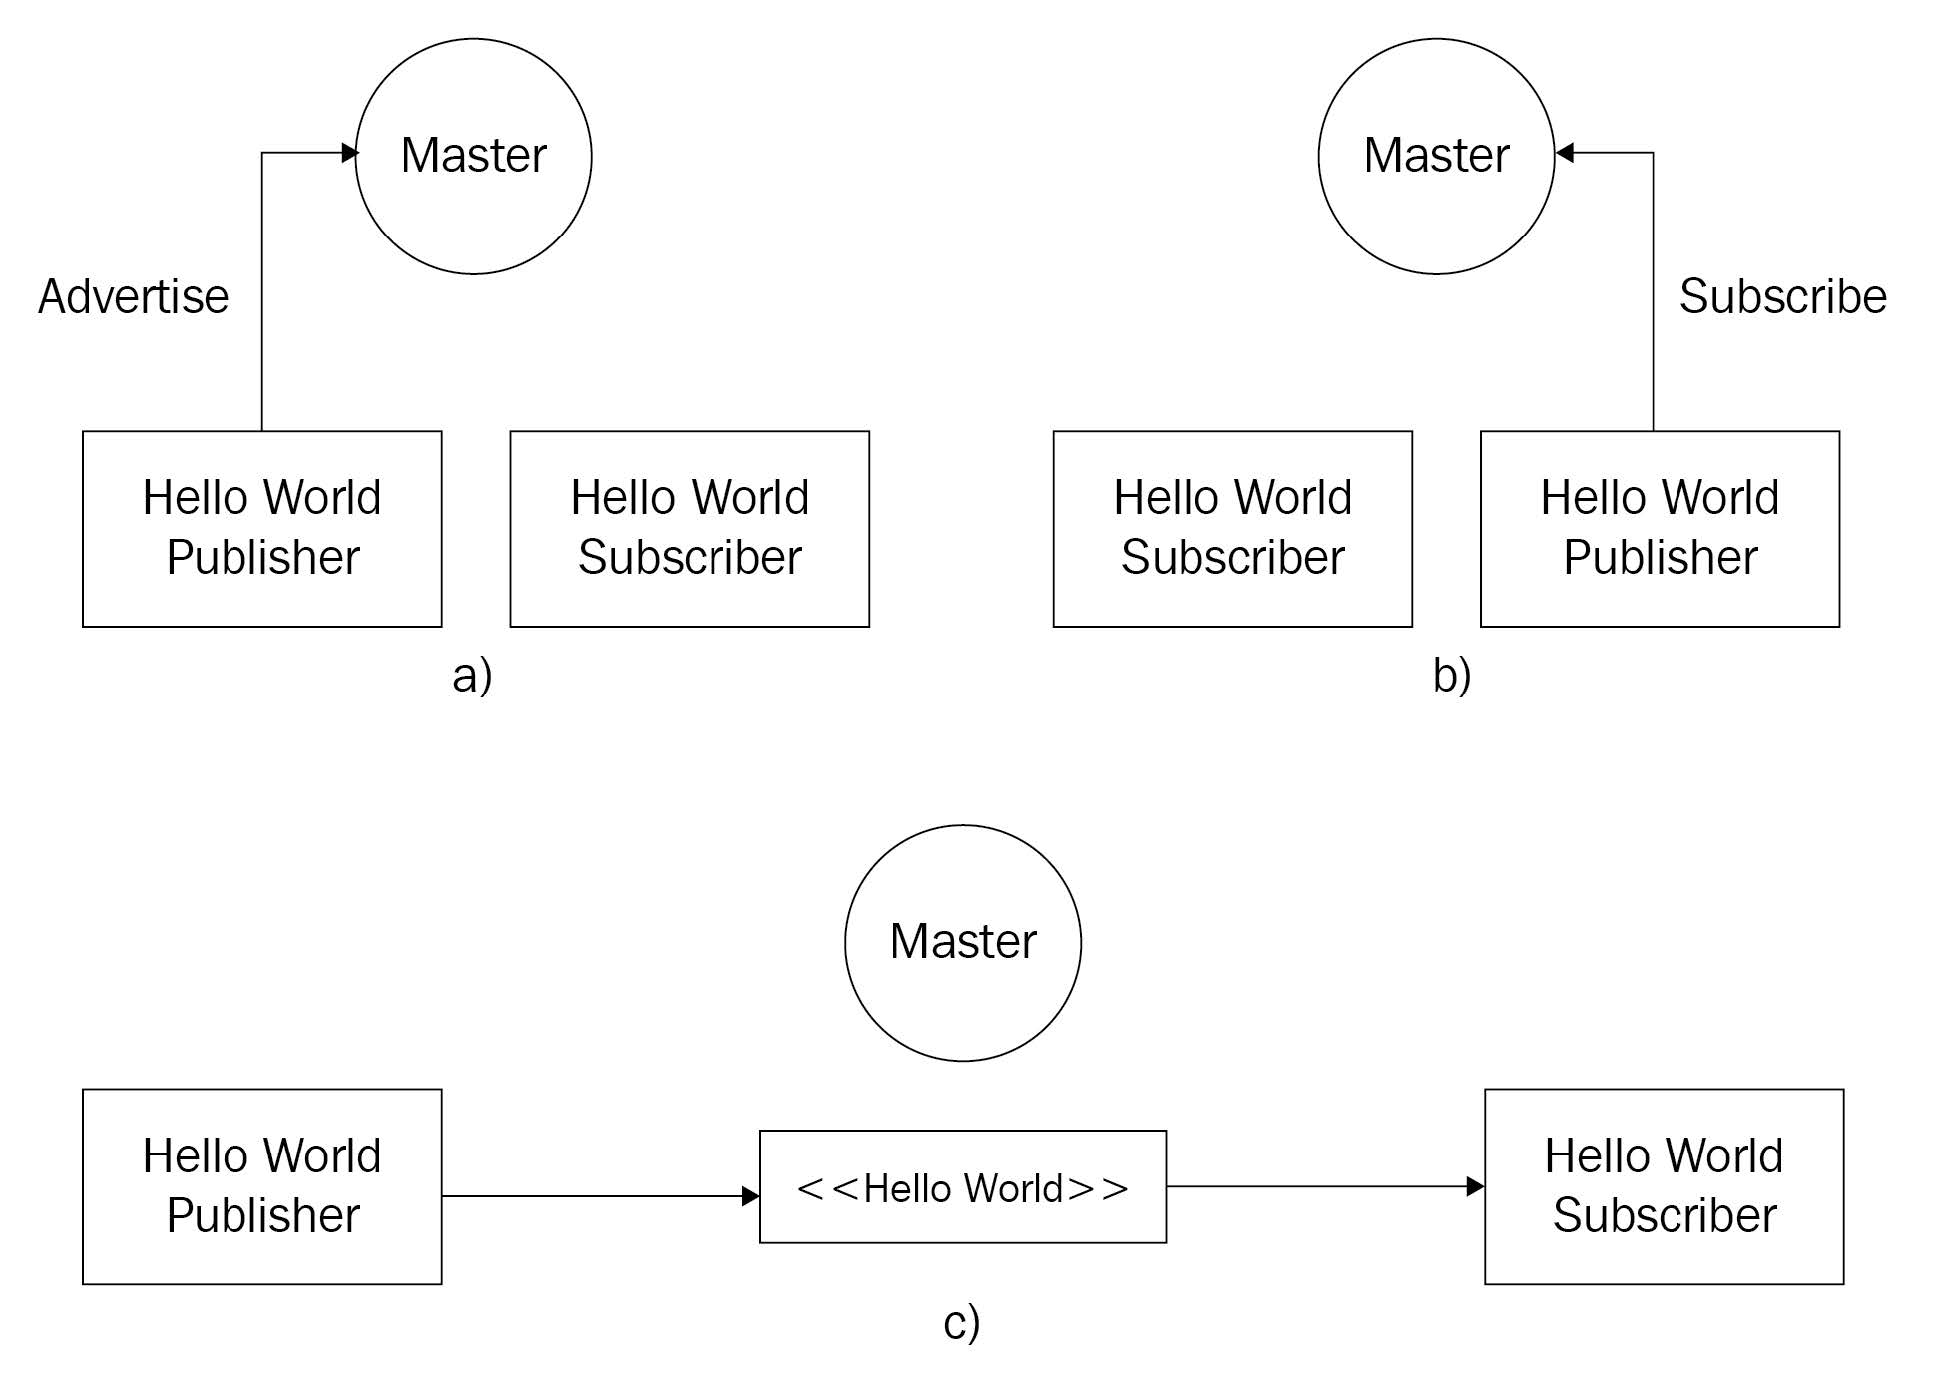
\includegraphics{img/helloWorld.jpg}
    \caption[ROS Communication Overview]{Communication between the ROS master and Hello World publisher and subscriber}
    \label{fig:helloWorld}
\end{figure}
When the publisher node starts advertising the \texttt{Hello World} message in a particular
topic, the ROS master gets the details of the topic and the node. It will check whether any
node is subscribing to the same topic. If no nodes are subscribing to the same topic at that
time, both nodes will remain unconnected. If the publisher and subscriber nodes run at
the same time, the ROS master will exchange the details of the publisher to the subscriber,
and they will connect and exchange data through ROS topics.
\subsection{ROS parameter}
When programming a robot, we might have to define robot parameters to tune
our control algorithm, such as the robot controller gains P, I, and D of a standard
proportional integral derivative controller. When the number of parameters increases,
we might need to store them as files. In some situations, these parameters must be shared
between two or more programs. In this case, ROS provides a parameter server, which is a
shared server in which all the ROS nodes can access parameters from this server. A node
can read, write, modify, and delete parameter values from the parameter server.

We can store these parameters in a file and load them into the server. The server can store a wide variety of data types and even dictionaries. The programmer can also set the scope of the parameter; that is, whether it can be accessed by only this node or all the nodes.

The parameter server supports the following XMLRPC data types:
\begin{itemize}
    \item 32-bit integers
    \item Booleans
    \item Strings
    \item Doubles
    \item ISO8601 dates
    \item Lists
    \item Base64-encoded binary data
\end{itemize}

We can also store dictionaries on the parameter server. If the number of parameters is high, we can use a YAML file to save them. Here is an example of the YAML file parameter definitions:

\begin{verbatim}
/camera/name : 'nikon' #string_type
/camera/fps : 30 #integer
/camera/exposure : 1.2 #float
/camera/active : true #boolean
\end{verbatim}

The \texttt{rosparam} tool is used to get and set the ROS parameter from the command line. The following are the commands for working with ROS parameters:
\begin{itemize}
    \item \texttt{rosparam set [parameter\_name] [value]}: This command will set a value in the given parameter.
    \item \texttt{rosparam get [parameter\_name]}: This command will retrieve a value from the given parameter.
    \item \texttt{rosparam load [YAML\_file]}: The ROS parameters can be saved into a YAML file. It can load them into the parameter server using this command.
    \item \texttt{rosparam dump [YAML\_file]}: This command will dump the existing ROS parameters into a YAML file.
    \item \texttt{rosparam delete [parameter\_name]}: This command will delete the given parameter.
    \item \texttt{rosparam list}: This command will list existing parameter names.
\end{itemize}
These parameters can be changed dynamically when you're executing a node that uses these parameters by using the \textbf{dynamic\_reconfigure} package (\url{http://wiki.ros.org/dynamic_reconfigure}).

\newpage
\subsection{ROS distributions}
ROS updates are released with new ROS distributions. A new distribution of ROS is composed of an updated version of its core software and a set of new/updated ROS packages. ROS follows the same release cycle as the Ubuntu Linux distribution: a new version of ROS is released every 6 months. Typically, for each Ubuntu LTS version, an \textbf{LTS} version of ROS is released. \textbf{Long Term Support (LTS)} and means that the released software will be maintained for a long time (5 years in the case of ROS and Ubuntu).

\begin{table}[h!]
\begin{tcolorbox}[
    colback=red!5!white,colframe=red!75!black,
    title={\textbf{Built-in Field Types for Message Definition}},
    fonttitle=\bfseries, coltitle=white, width=\linewidth
]
    \centering
    \renewcommand{\arraystretch}{1} % Increase row height for better alignment
    \begin{longtable}{|
        >{\centering\arraybackslash}m{2.5cm}|
        >{\centering\arraybackslash}m{2cm}|
        >{\centering\arraybackslash}m{3cm}|
        >{\centering\arraybackslash}m{1.5cm}|
        >{\centering\arraybackslash}m{3cm}|}
    \hline 
    \rowcolor{red!20}
    \textbf{Distro} & \textbf{Release date} & \textbf{Poster} & \textbf{Turtle} & \textbf{EOL date} \\
    \hline \midrule

    ROS Noetic Ninjemys (Recommended) & May 23rd, 2020 & 
    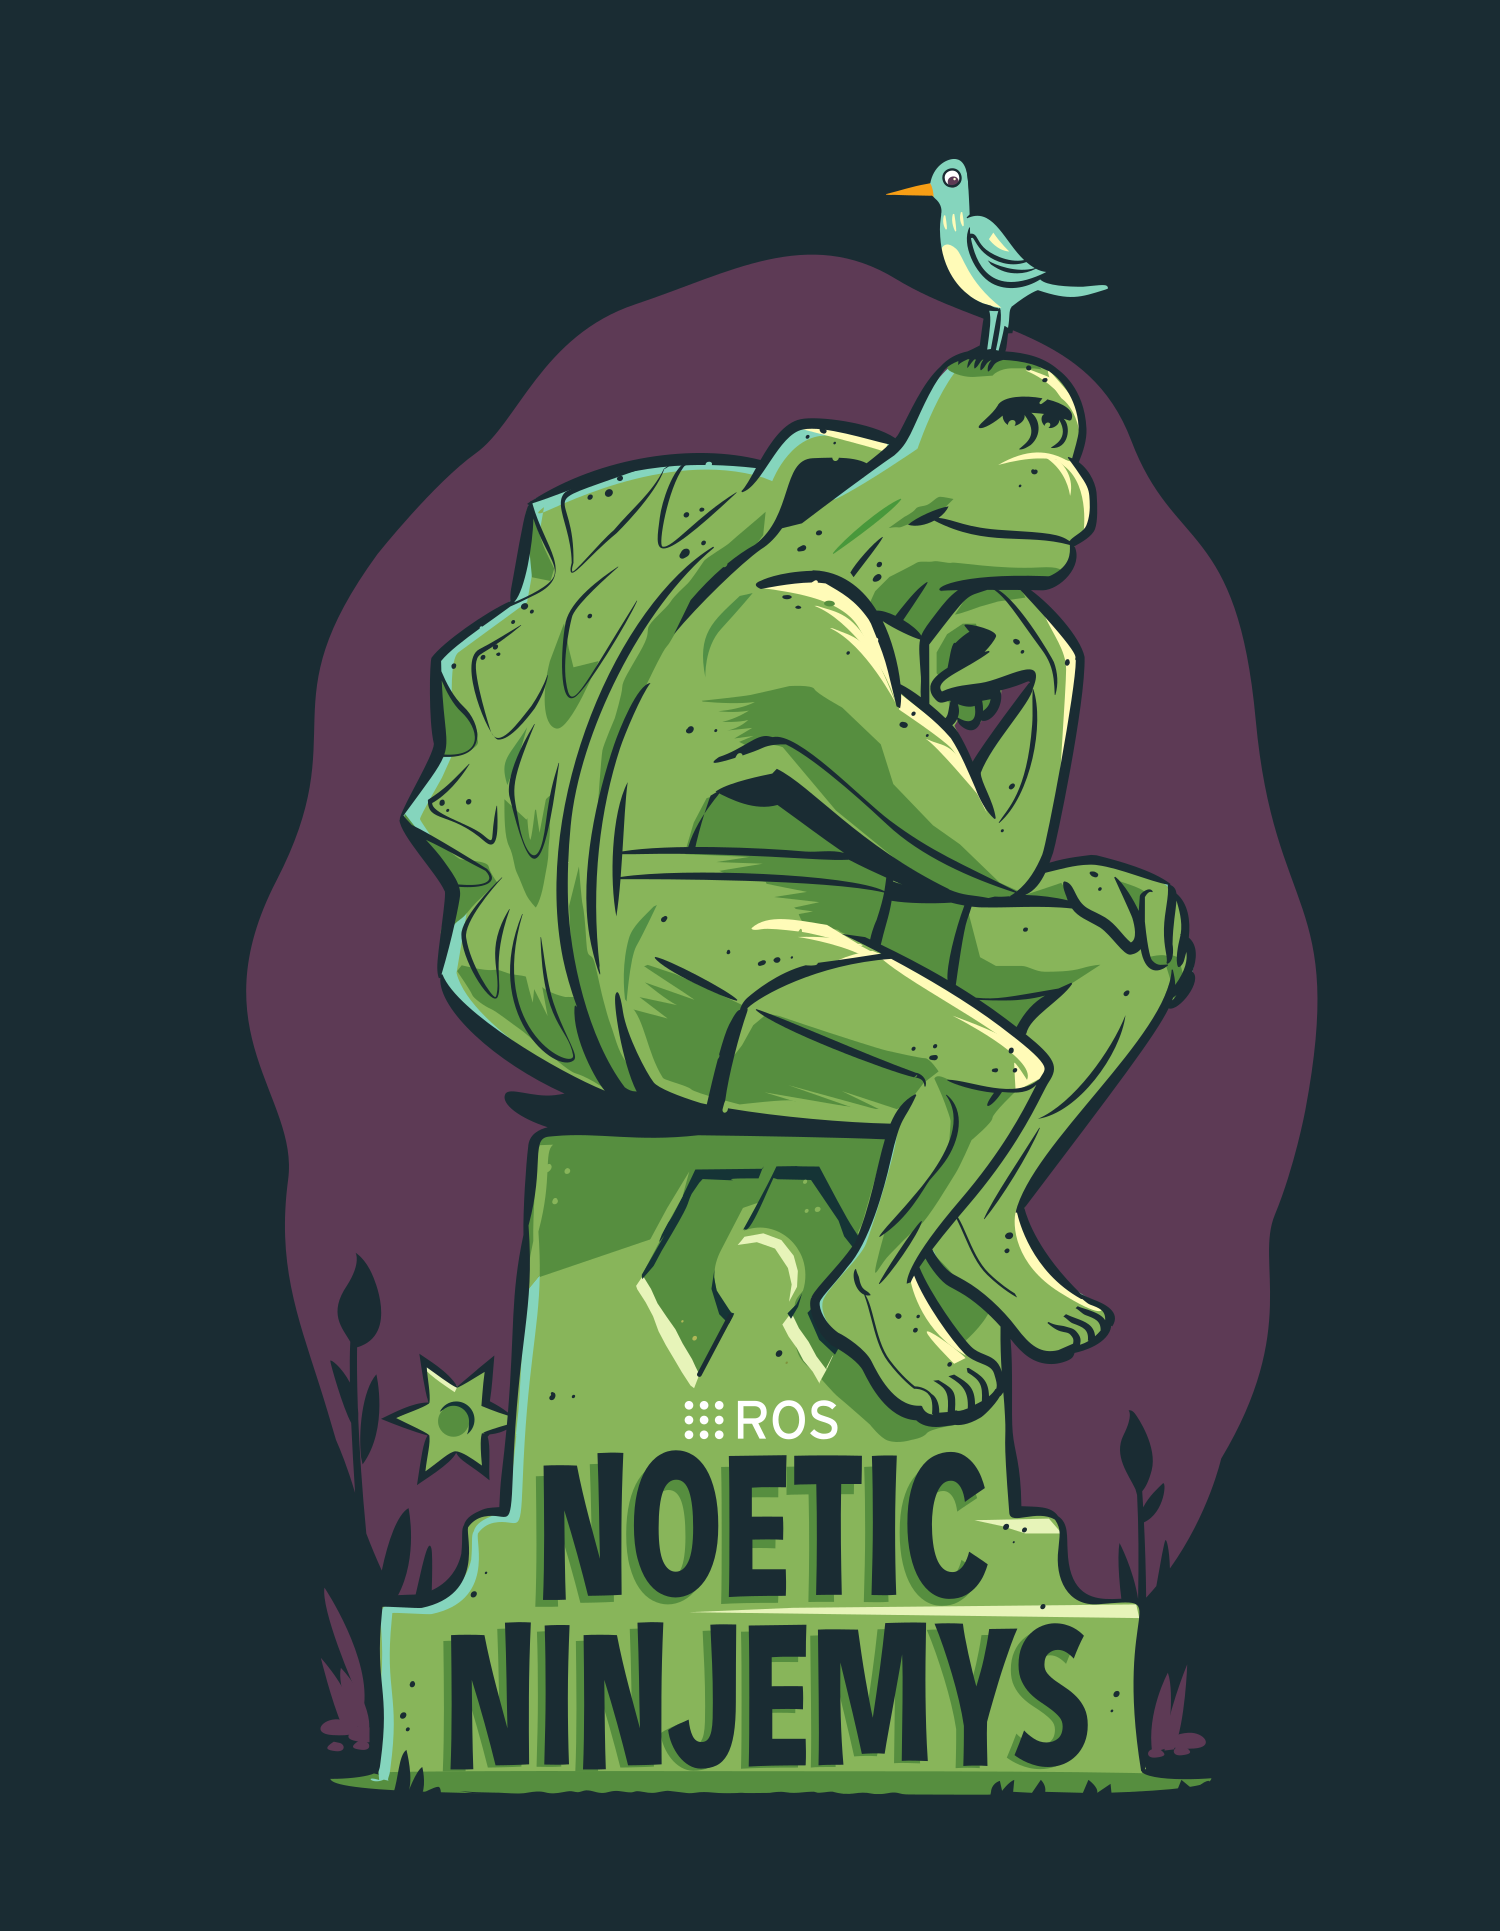
\includegraphics[width=0.18\textwidth]{img/noetic.png} & 
    
\includegraphics[width=0.08\textwidth]{img/noetic_c.png} & 
    May, 2025 (Focal EOL) \\ \hline

    ROS Melodic Morenia & May 23rd, 2018 & 
    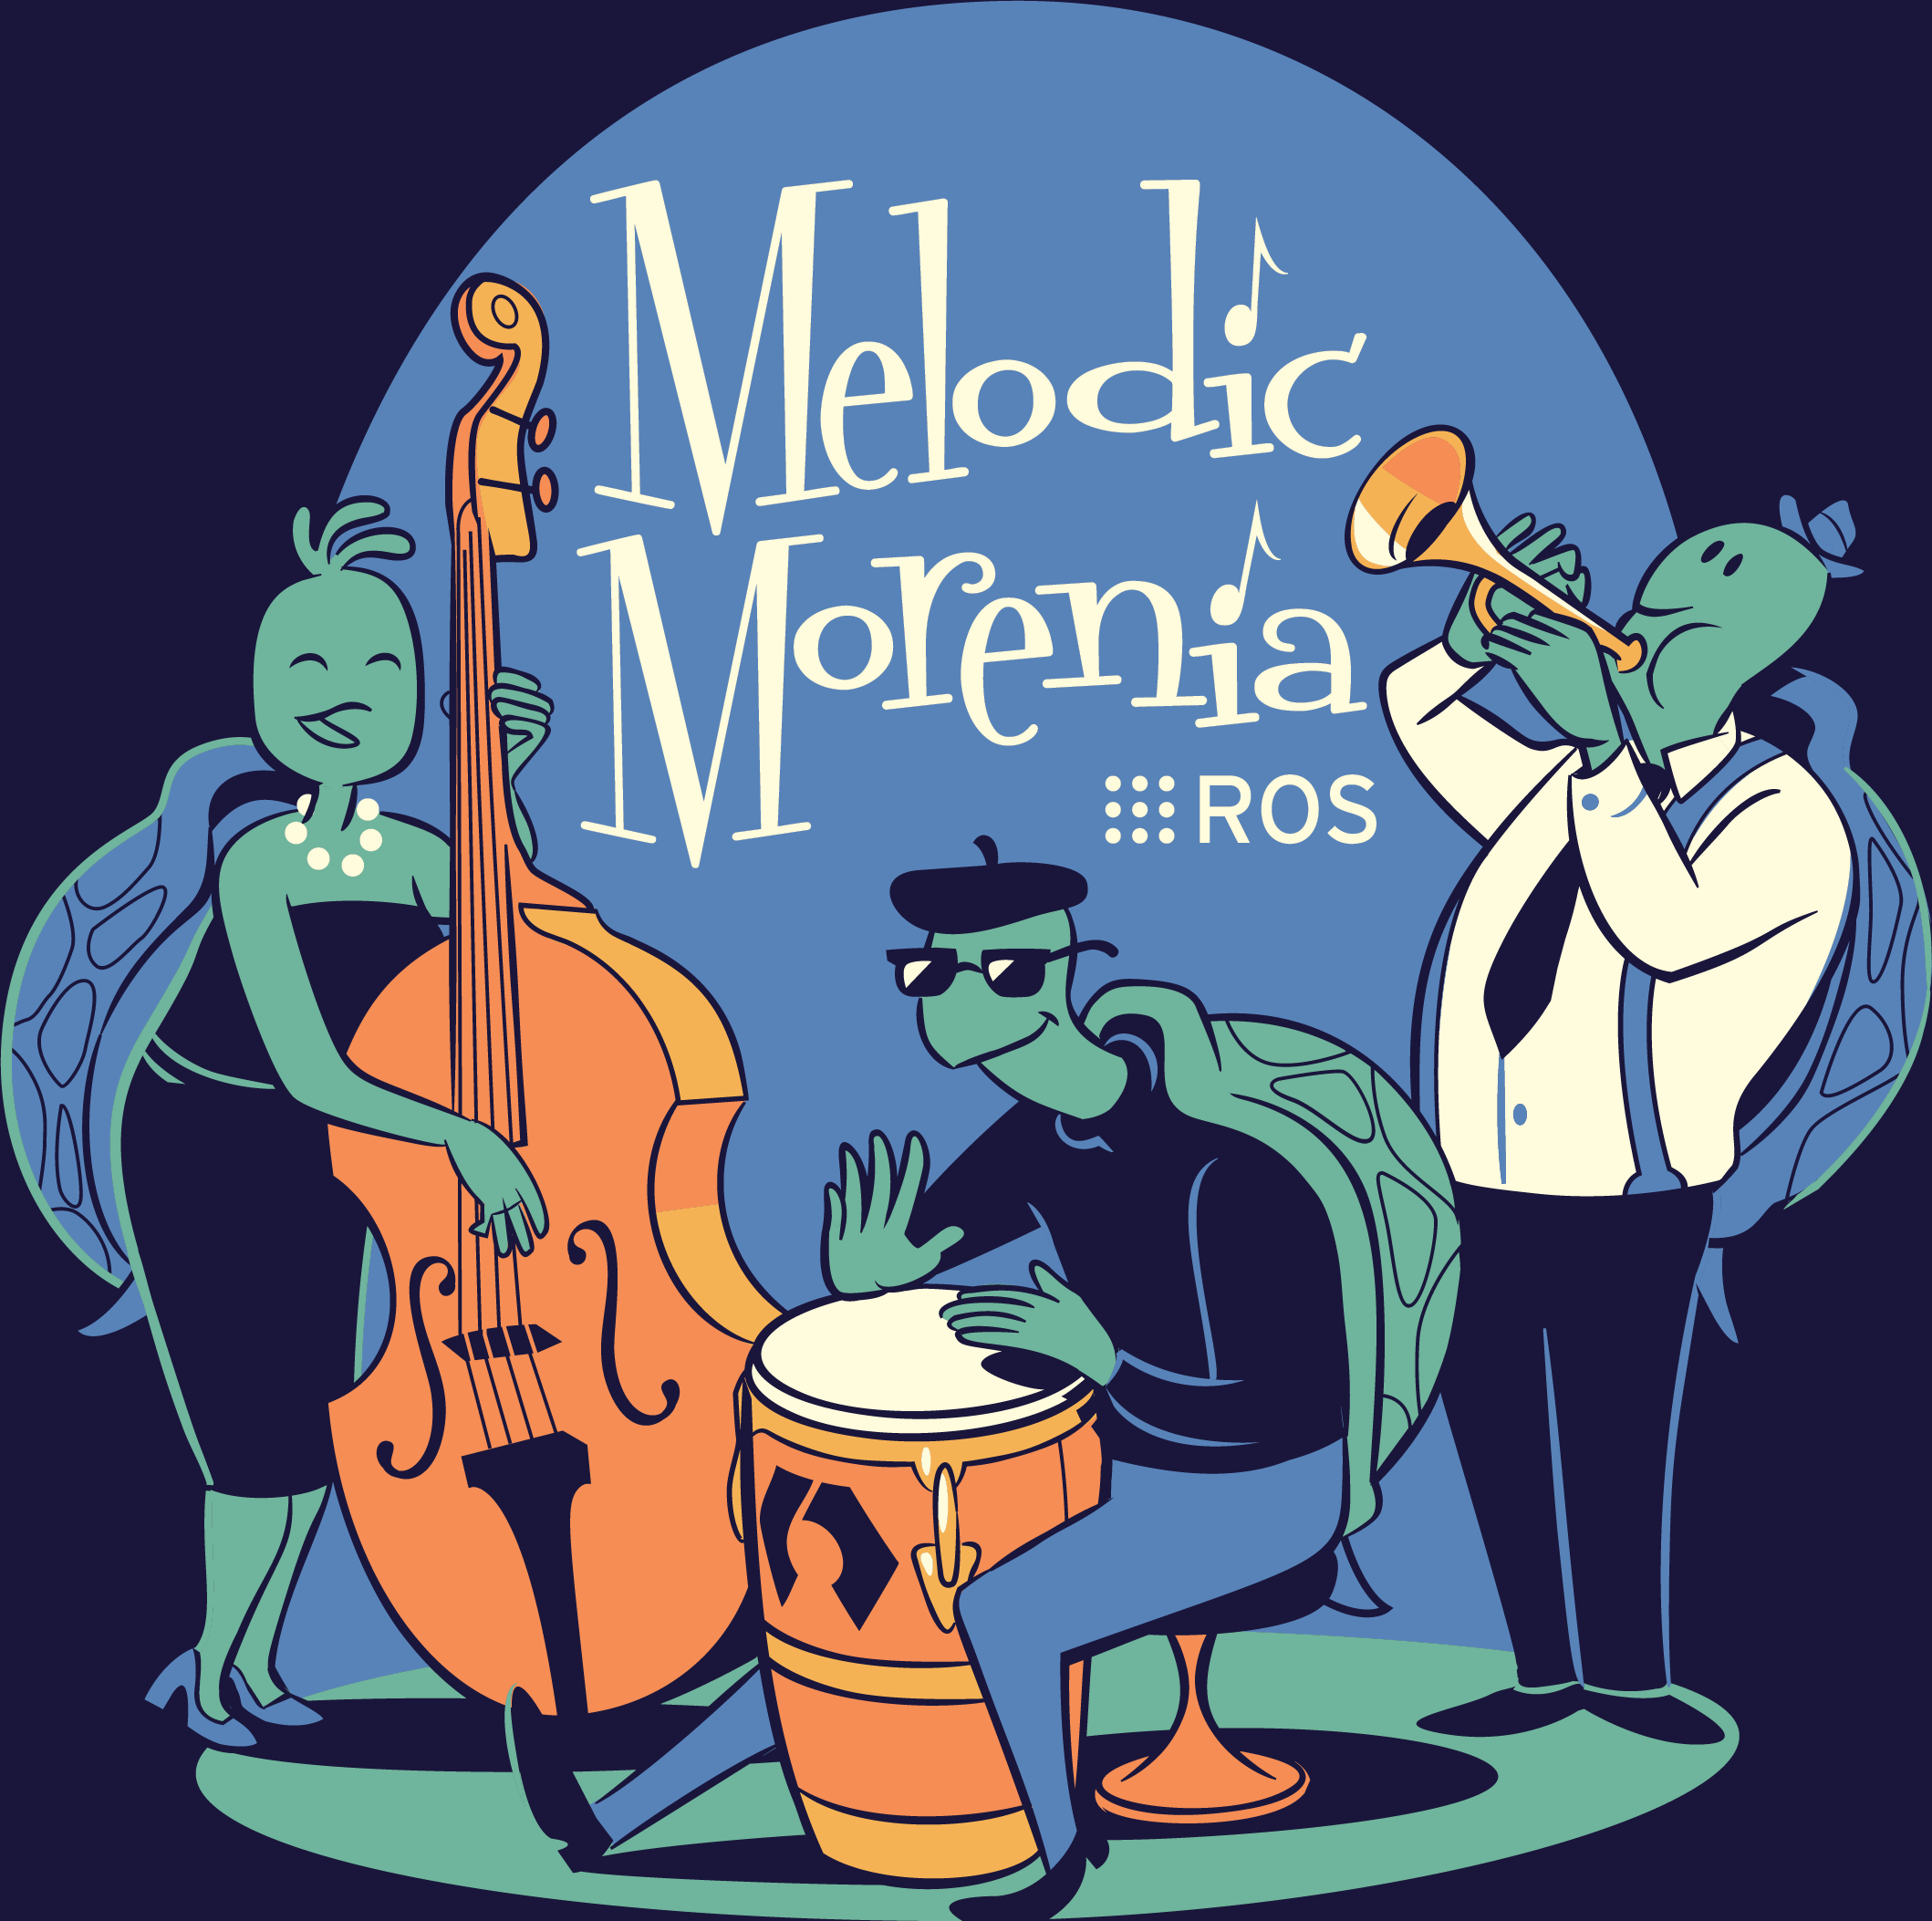
\includegraphics[width=0.18\textwidth]{img/melodic_with_bg.png} & 
    
\includegraphics[width=0.08\textwidth]{img/melodic.png} & 
    June 27, 2023 (Bionic EOL) \\ \hline

    ROS Lunar Loggerhead & May 23rd, 2017 & 
    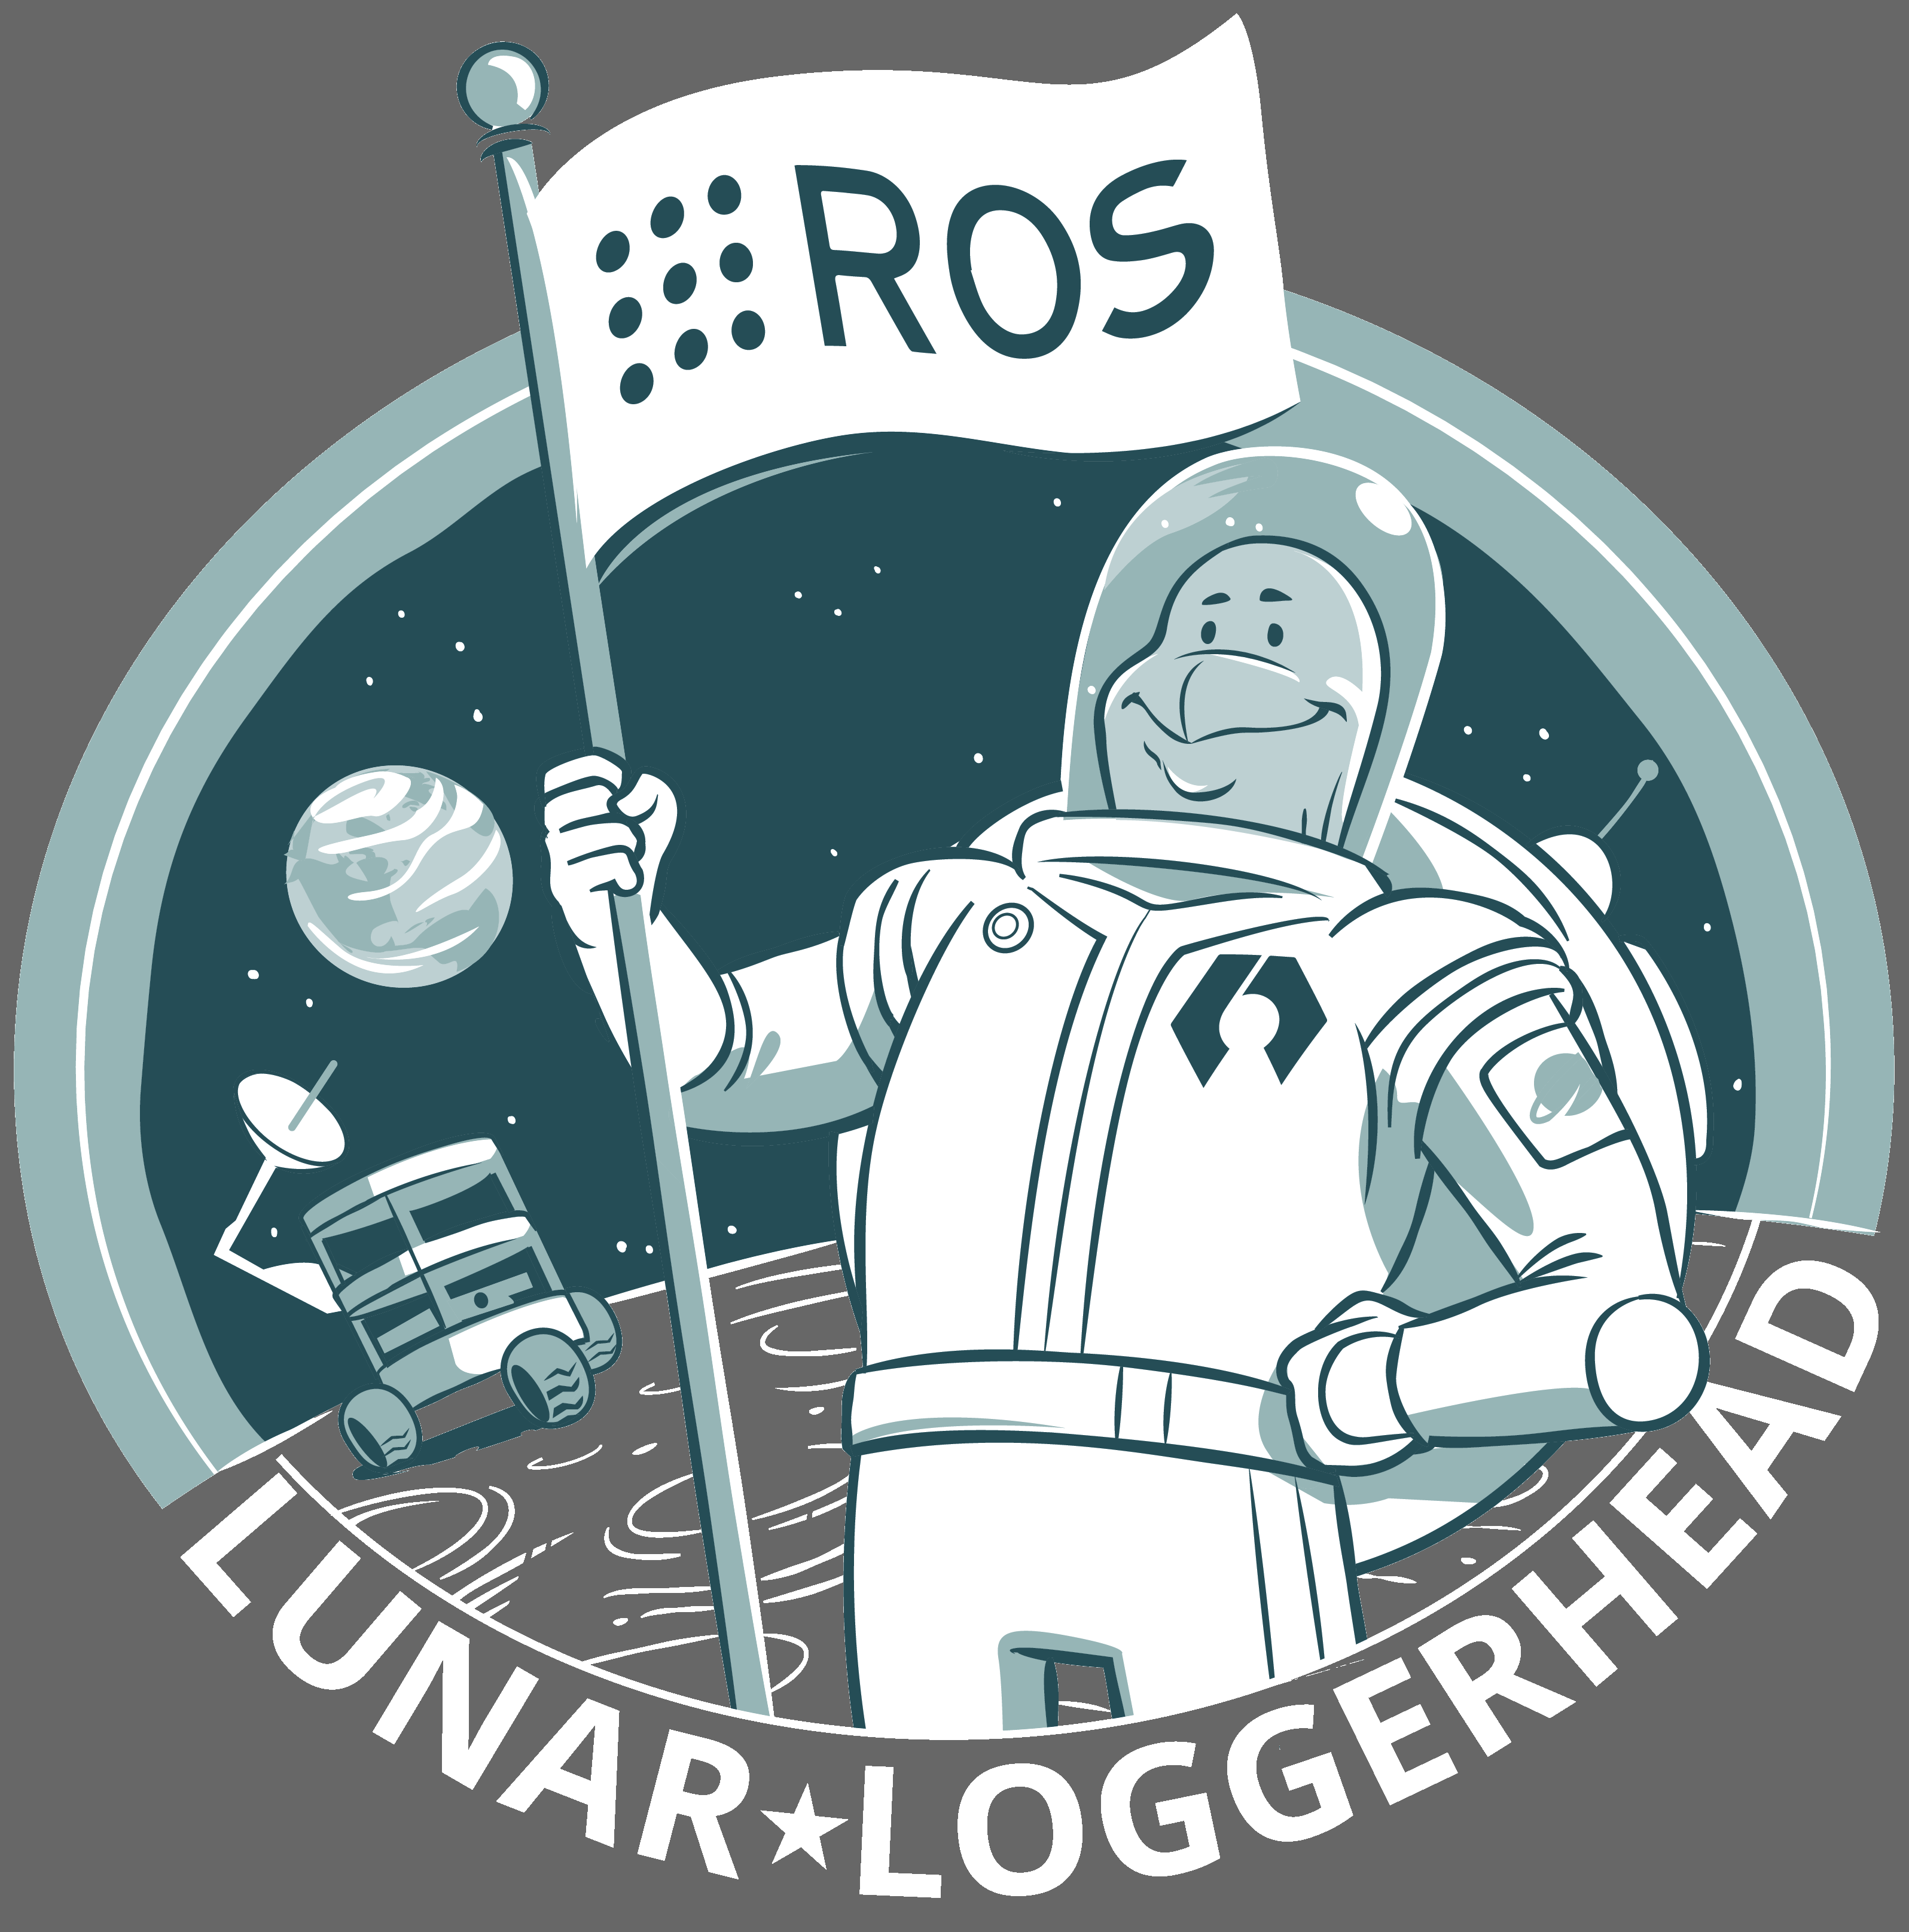
\includegraphics[width=0.18\textwidth]{img/lunar_with_bg.png} & 
    
\includegraphics[width=0.08\textwidth]{img/lunar.png} & 
    May, 2019 \\ \hline

    ROS Kinetic Kame & May 23rd, 2016 & 
    
\includegraphics[width=0.18\textwidth]{img/kinetic.png} & 
    
\includegraphics[width=0.08\textwidth]{img/kinetic (1).png} & 
    April, 2021 (Xenial EOL) \\ \hline

    \end{longtable}
\end{tcolorbox}
\caption{ROS Distributions Table}
\end{table}
\newpage
\subsection{Running the ROS master and the ROS parameter
server}
Before running any ROS nodes, we should start the ROS master and the ROS parameter server. We can start the ROS master and the ROS parameter server by using a single command called \textbf{roscore}, which will start the following programs:
\begin{itemize}
    \item \texttt{ROS master}
    \item \texttt{ROS parameter server}
    \item \texttt{rosout logging nodes}
\end{itemize}

The rosout node will collect log messages from other ROS nodes and store them in a log file, and will also re-broadcast the collected log message to another topic. The /rosout topic is published by ROS nodes using ROS client libraries such as roscpp and rospy, and this topic is subscribed by the rosout node, which rebroadcasts the message in another topic called /rosout\_agg. This topic contains an aggregate stream of log messages. The roscore command should be run as a prerequisite to running any ROS nodes. The following screenshot shows the messages that are printed when we run the roscore command in a Terminal.

Use the following command to run \texttt{roscore} on a Linux Terminal:
\begin{codebox}[]{Starting the ROS Master}    
    \begin{minted}{bash}
        roscore
    \end{minted}
\end{codebox}

After running this command, we will see the following text in the Linux Terminal:
\begin{figure}[ht]
    \centering
    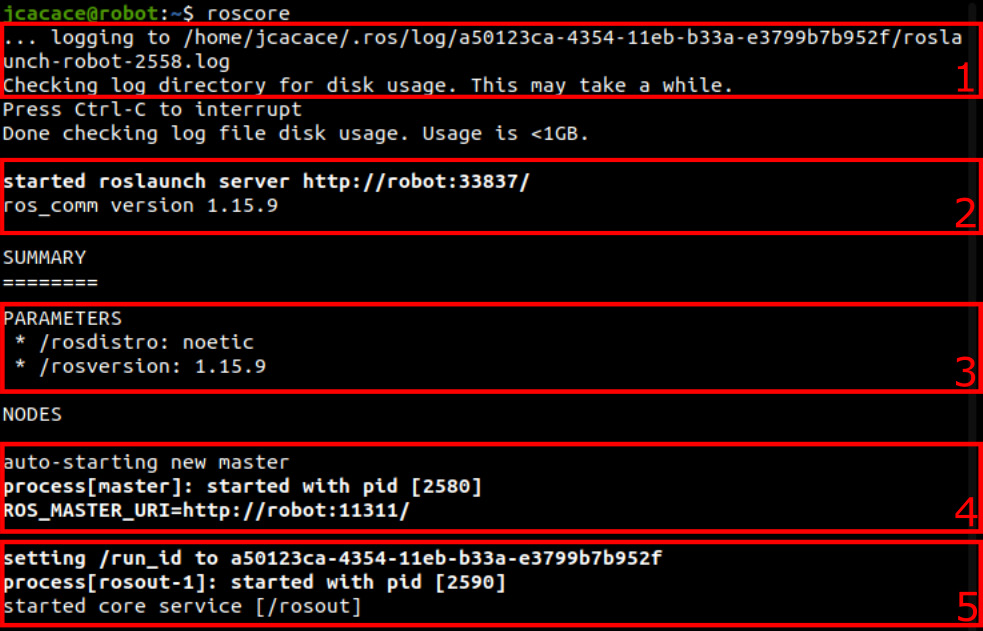
\includegraphics{img/roscore.jpg}
    \caption{Terminal messages while running the roscore command}
\end{figure}
\newpage
\begin{itemize}
    \item In section 1, we can see that a log file is created inside the \textasciitilde/.ros/log folder for collecting logs from ROS nodes. This file can be used for debugging purposes.
    \item In section 2, the command starts a ROS launch file called \texttt{roscore.xml}. When a launch file starts, it automatically starts \texttt{rosmaster} and the ROS parameter server. The \texttt{roslaunch} command is a Python script, which can start \texttt{rosmaster} and the ROS parameter server whenever it tries to execute a launch file. This section shows the address of the ROS parameter server within the port.
    \item In section 3, we can see parameters such as \texttt{rosdistro} and \texttt{rosversion} being displayed in the Terminal. These parameters are displayed when it executes \texttt{roscore.xml}. We will look at \texttt{roscore.xml} in more detail in the next section.
    \item In section 4, we can see that the \texttt{rosmaster} node is being started with \texttt{ROS\_MASTER\_URI}, which we defined earlier as an environment variable.
    \item In section 5, we can see that the \texttt{rosout} node is being started, which will start subscribing to the \texttt{/rosout} topic and rebroadcasting it to \texttt{/rosout\_agg}.
\end{itemize}

The following is the content of \texttt{roscore.xml}:
\begin{codebox}[]{Output of the roscore Command and the Structure of roscore.xml}
    
    \begin{minted}{xml}
    <launch>
        <group ns="/">
            <param name="rosversion" command="rosversion roslaunch" />
            <param name="rosdistro" command="rosversion -d" />
            <node pkg="rosout" type="rosout" name="rosout" respawn="true"/>
        </group>
    </launch>
\end{minted}
    \end{codebox}

When the \texttt{roscore} command is executed, initially, the command checks the command-line argument for a new port number for \texttt{rosmaster}. If it gets the port number, it will start listening to the new port number; otherwise, it will use the default port. This port number and the \texttt{roscore.xml} launch file will be passed to the \texttt{roslaunch} system. The \texttt{roslaunch} system is implemented in a Python module; it will parse the port number and launch the \texttt{roscore.xml} file.

In the \texttt{roscore.xml} file, we can see that the ROS parameters and nodes are encapsulated in a group XML tag with a \texttt{/} namespace. The group XML tag indicates that all the nodes inside this tag have the same settings.


The \texttt{rosversion} and \texttt{rosdistro} parameters store the output of the \\ \texttt{rosversion roslaunch} and \texttt{rosversion -d} commands using the \texttt{command} tag, which is a part of the ROS param tag. The \texttt{command} tag will execute the command mentioned in it and store the output of the command in these two parameters.

\texttt{rosmaster} and the parameter server are executed inside \texttt{roslaunch} modules via the \texttt{ROS\_MASTER\_URI} address. This happens inside the \texttt{roslaunch} Python module.\\ \texttt{ROS\_MASTER\_URI} is a combination of the IP address and port that \texttt{rosmaster} is going to listen to. The port number can be changed according to the given port number in the \texttt{roscore} command.

\subsubsection{Checking the roscore command's output}
Let's check out the ROS topics and ROS parameters that are created after running roscore. The following command will list the active topics in the Terminal:

\begin{codebox}[]{Listing Active Topics After Running the roscore Command}    
    \begin{minted}{bash}
        rostopic list
    \end{minted}
    \end{codebox}

The list of topics is as follows, as per our discussion of the rosout node's subscribe /rosout topic. This contains all the log messages from the ROS nodes. /rosout\_agg will rebroadcast the log messages:

\begin{codebox}[]{Active Topics After Running roscore: /rosout and /rosout\_agg}    
    \begin{minted}{bash}
        /rosout
        /rosout_agg
    \end{minted}
    \end{codebox}

The following command lists the parameters that are available when running roscore. The following command is used to list the active ROS parameter:

\begin{codebox}[]{Listing Active ROS Parameters After Running roscore}    
    \begin{minted}{bash}
        rosparam list
    \end{minted}
    \end{codebox}

These parameters are mentioned here; they provide the ROS distribution name, version, the address of the roslaunch server, and run\_id, where run\_id is a unique ID associated with a particular run of roscore:
\begin{codebox}[]{ROS Parameters Available After Running roscore}
    
    \begin{minted}{bash}
        /rosdistro
        /roslaunch/uris/host_robot_virtualbox_51189
        /rosversion
        /run_id
    \end{minted}
    \end{codebox}

The list of ROS services that's generated when running roscore can be checked by using the following command:

\begin{codebox}[]{Listing ROS Services Generated by roscore}
    \begin{minted}{bash}
        rosservice list
    \end{minted}
    \end{codebox}

The list of services that are running is as follows:

\begin{codebox}[]{Active ROS Services After Running roscore}
    
    \begin{minted}{bash}
        /rosout/get_loggers
        /rosout/set_logger_level
    \end{minted}
    \end{codebox}


These ROS services are generated for each ROS node, and they are used to set the logging
levels.
\end{document}